
\begin{figure}[!ht]
\begin{center}
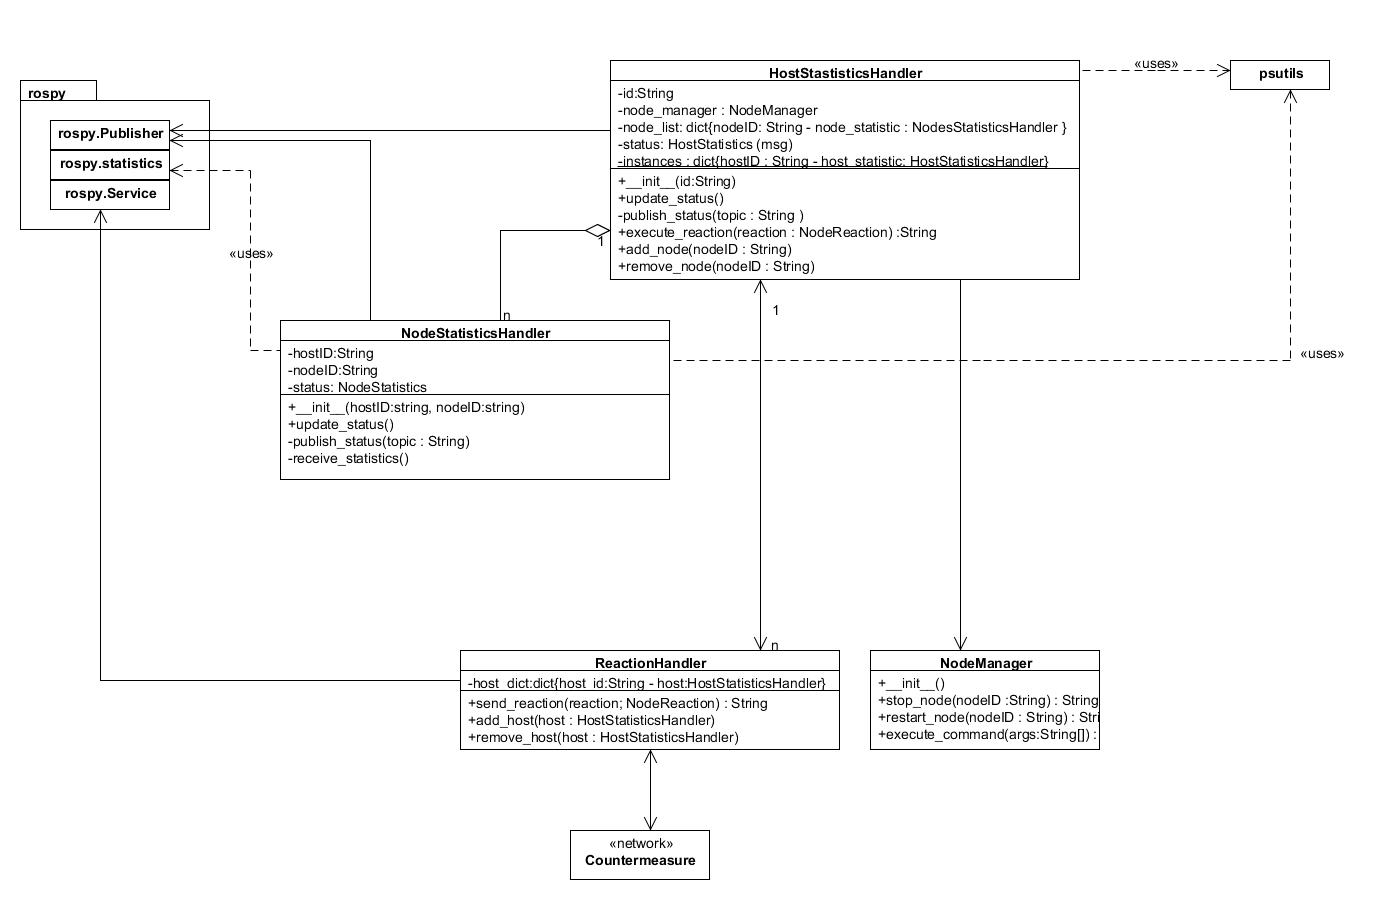
\includegraphics[width = 1.0 \linewidth]{./diagram_pictures/erfassung.jpg}
\caption{UML diagram of the NodeInterface package}
\end{center}
\end{figure}
\newpage

\subsection{HostStatisticsHandler}
Represents a host . Limited to one instance per host. Collects statistics about the current state of the host and sends them using the publisher-subscriber mechanism.

\subsubsection{Attributes}
\begin{itemize}
	\item \textbf{private string id}\\
			ip of the host.
	\item \textbf{private NodeManager node\_manager}\\
			NodeManager providing function to restart and stop Nodes.
	\item \textbf{private  dict\{String nodeID  - NodesStatisticsHandler node\_statistic  \} node\_list}\\
			Dictionary holding all Nodes and their statistics, currently running on the host.
	\item \textbf{private HostStatistics status}\\
			Holds the current statistics about the  status of the host.
	\item \textbf{private static dict\{String hostID   - HostStatisticsHandler host\_statistic \}}\\
			Holds references to all initiated host, to prevent multiple instances of a single host.
\end{itemize}

\subsubsection{Methods}
\begin{itemize}
	\item \textbf{public void update\_status()}\\
			collects statistics about the host's current status using psutils.
	\item \textbf{private void publish\_status(String topic)}\\
			publishes the current status to a topic using ROS's publisher-subscriber mechanism.
	\item \textbf{public String execute\_reaction(NodeReaction reaction)}\\
			parses through the reaction and calls the appropriate method from the NodeManager.
			Returns a message about operation's success.
	\item \textbf{public void add\_node(String nodeID)}\\
			adds a Node with the given id to the host.
	\item \textbf{public void remove\_node(String nodeID)}\\
			removes the Node with the given id from the host.
\end{itemize}

\subsection{NodeStatisticsHandler}
Holds the statistics of an individual Node.

\subsubsection{Attributes}
\begin{itemize}
	\item \textbf{private String hostID}\\
	id of the host this node runs on
	\item \textbf{private String nodeID}\\
	identifier of this node
	\item \textbf{private NodeStatistics status}\\
	current statistcs about the status of the node
\end{itemize}

\subsubsection{Methods}
\begin{itemize}
	\item \textbf{public void update\_status()}\\
	collects statistics about the node's current status using psutils and rospy.statistics
	\item \textbf{private void publish\_status()}\\
	publishes the current status to a topic using ROS's publisher-subscriber mechanism.
	\item \textbf{private void receive\_statistics()}\\
	receives the statistics published by ROS Topic statistics
\end{itemize}

\subsection{NodeManager}
can restart or stop nodes or execute a countermeasure 

\subsubsection{Methods}
\begin{itemize}
	\item \textbf{public String stop\_node(String nodeID)}\\
	stops the node with the given id.
	Returns a message about operation's success.
	\item \textbf{public String restart\_node(String nodeID)}\\
	restarts a node with the given id.
	Returns a message about operation's success.
	\item \textbf{public String execute\_command(String[] args)}\\
	executes a system call with the given arguments.
	Returns a message about operation's success.
\end{itemize}

\subsection{ReactionHandler}
delegates the countermeasure to the concerned host.

\subsubsection{Attributes}
\begin{itemize}
	\item \textbf{private  dict\{String host\_id  - HostStatisticsHandler host  \} host\_dict}\\
	Dictionary of all hosts running on the network
\end{itemize}

\subsubsection{Methods}
\begin{itemize}
	\item \textbf{public String send\_reaction(NodeReaction reaction)}\\
	parses the reaction and delegates it to the concerned host.
	Returns a message about operation's success using rospy.Service
	\item \textbf{public void add\_host(HostStatisticsHandler host)}\\
	adds a host to the dictionary
	\item \textbf{public void remove\_host(HostStatisticsHandler host)}\\
	removes a host from the dictionary
\end{itemize}
	
\subsection{psutils}
library to acquire the system's usage statistics. For a more in-depth documentation, see the official psutils documentation.

\subsubsection{Used methods}
\begin{itemize}
	\item \textbf{psutil.cpu\_percent(interval, boolean percpu)}\\
	Return a float representing the current system-wide CPU usage.
	\item \textbf{psutil.virtual\_memory()}\\
	Return statistics about system memory usage.
	\item \textbf{psutil.net\_io\_counters(boolean pernic)}\\
	Return system-wide network I/O statistics.
	\item \textbf{psutil.disk\_usage(String path)}\\
	Return disk usage statistics about the given path.
	\item \textbf{psutil.disk\_io\_counters(boolean perdisk)}
	Return system-wide disk I/O statistics.
	\item \textbf{psutil.disk\_partitions()}\\
	Return all mounted disk partitions as a list of namedtuples.
	\item \textbf{psutil.Process(pid )}\\
	Represents an  process with the given pid
\end{itemize}


	